\section{The Quality of Reasoning CoTs Enhanced by RLVR}

% In addition to the LLM-as-a-CoT-Judge approach to strictly identify whether a reasoning CoT contains any critical error, we further leverage supervised fine-tuning (SFT) to measure the quality of reasoning CoTs enhanced by RLVR.
% Given training questions in DAPO, we conduct multiple SFT procedures starting from the same base LLM but learning CoTs generated by different models.
% If the CoT data is of high quality, we expect the post-SFT model would demonstrate better generalization performance.
% Figure~\ref{fig:cot_quality_analysis} includes the overall quality evaluation of different CoT data.

In addition to the LLM-as-a-CoT-Judge approach for strictly identifying critical errors in reasoning CoTs, we further leverage supervised fine-tuning (SFT) to assess the quality of reasoning CoTs enhanced by RLVR.
Given the training questions in DAPO, we conduct multiple SFT procedures, starting from the same base LLM and learning from CoTs generated by different models. If the CoT data is of high quality, we expect the post-SFT model to exhibit improved generalization performance. Figure~\ref{fig:cot_quality_analysis} presents an overall quality evaluation of various CoT data.

\begin{figure*}[t]
\centering
    \subfigure[
    The CoT quality at different RLVR stages, using Pass@1 on test sets as the proxy metric.
    ]{
        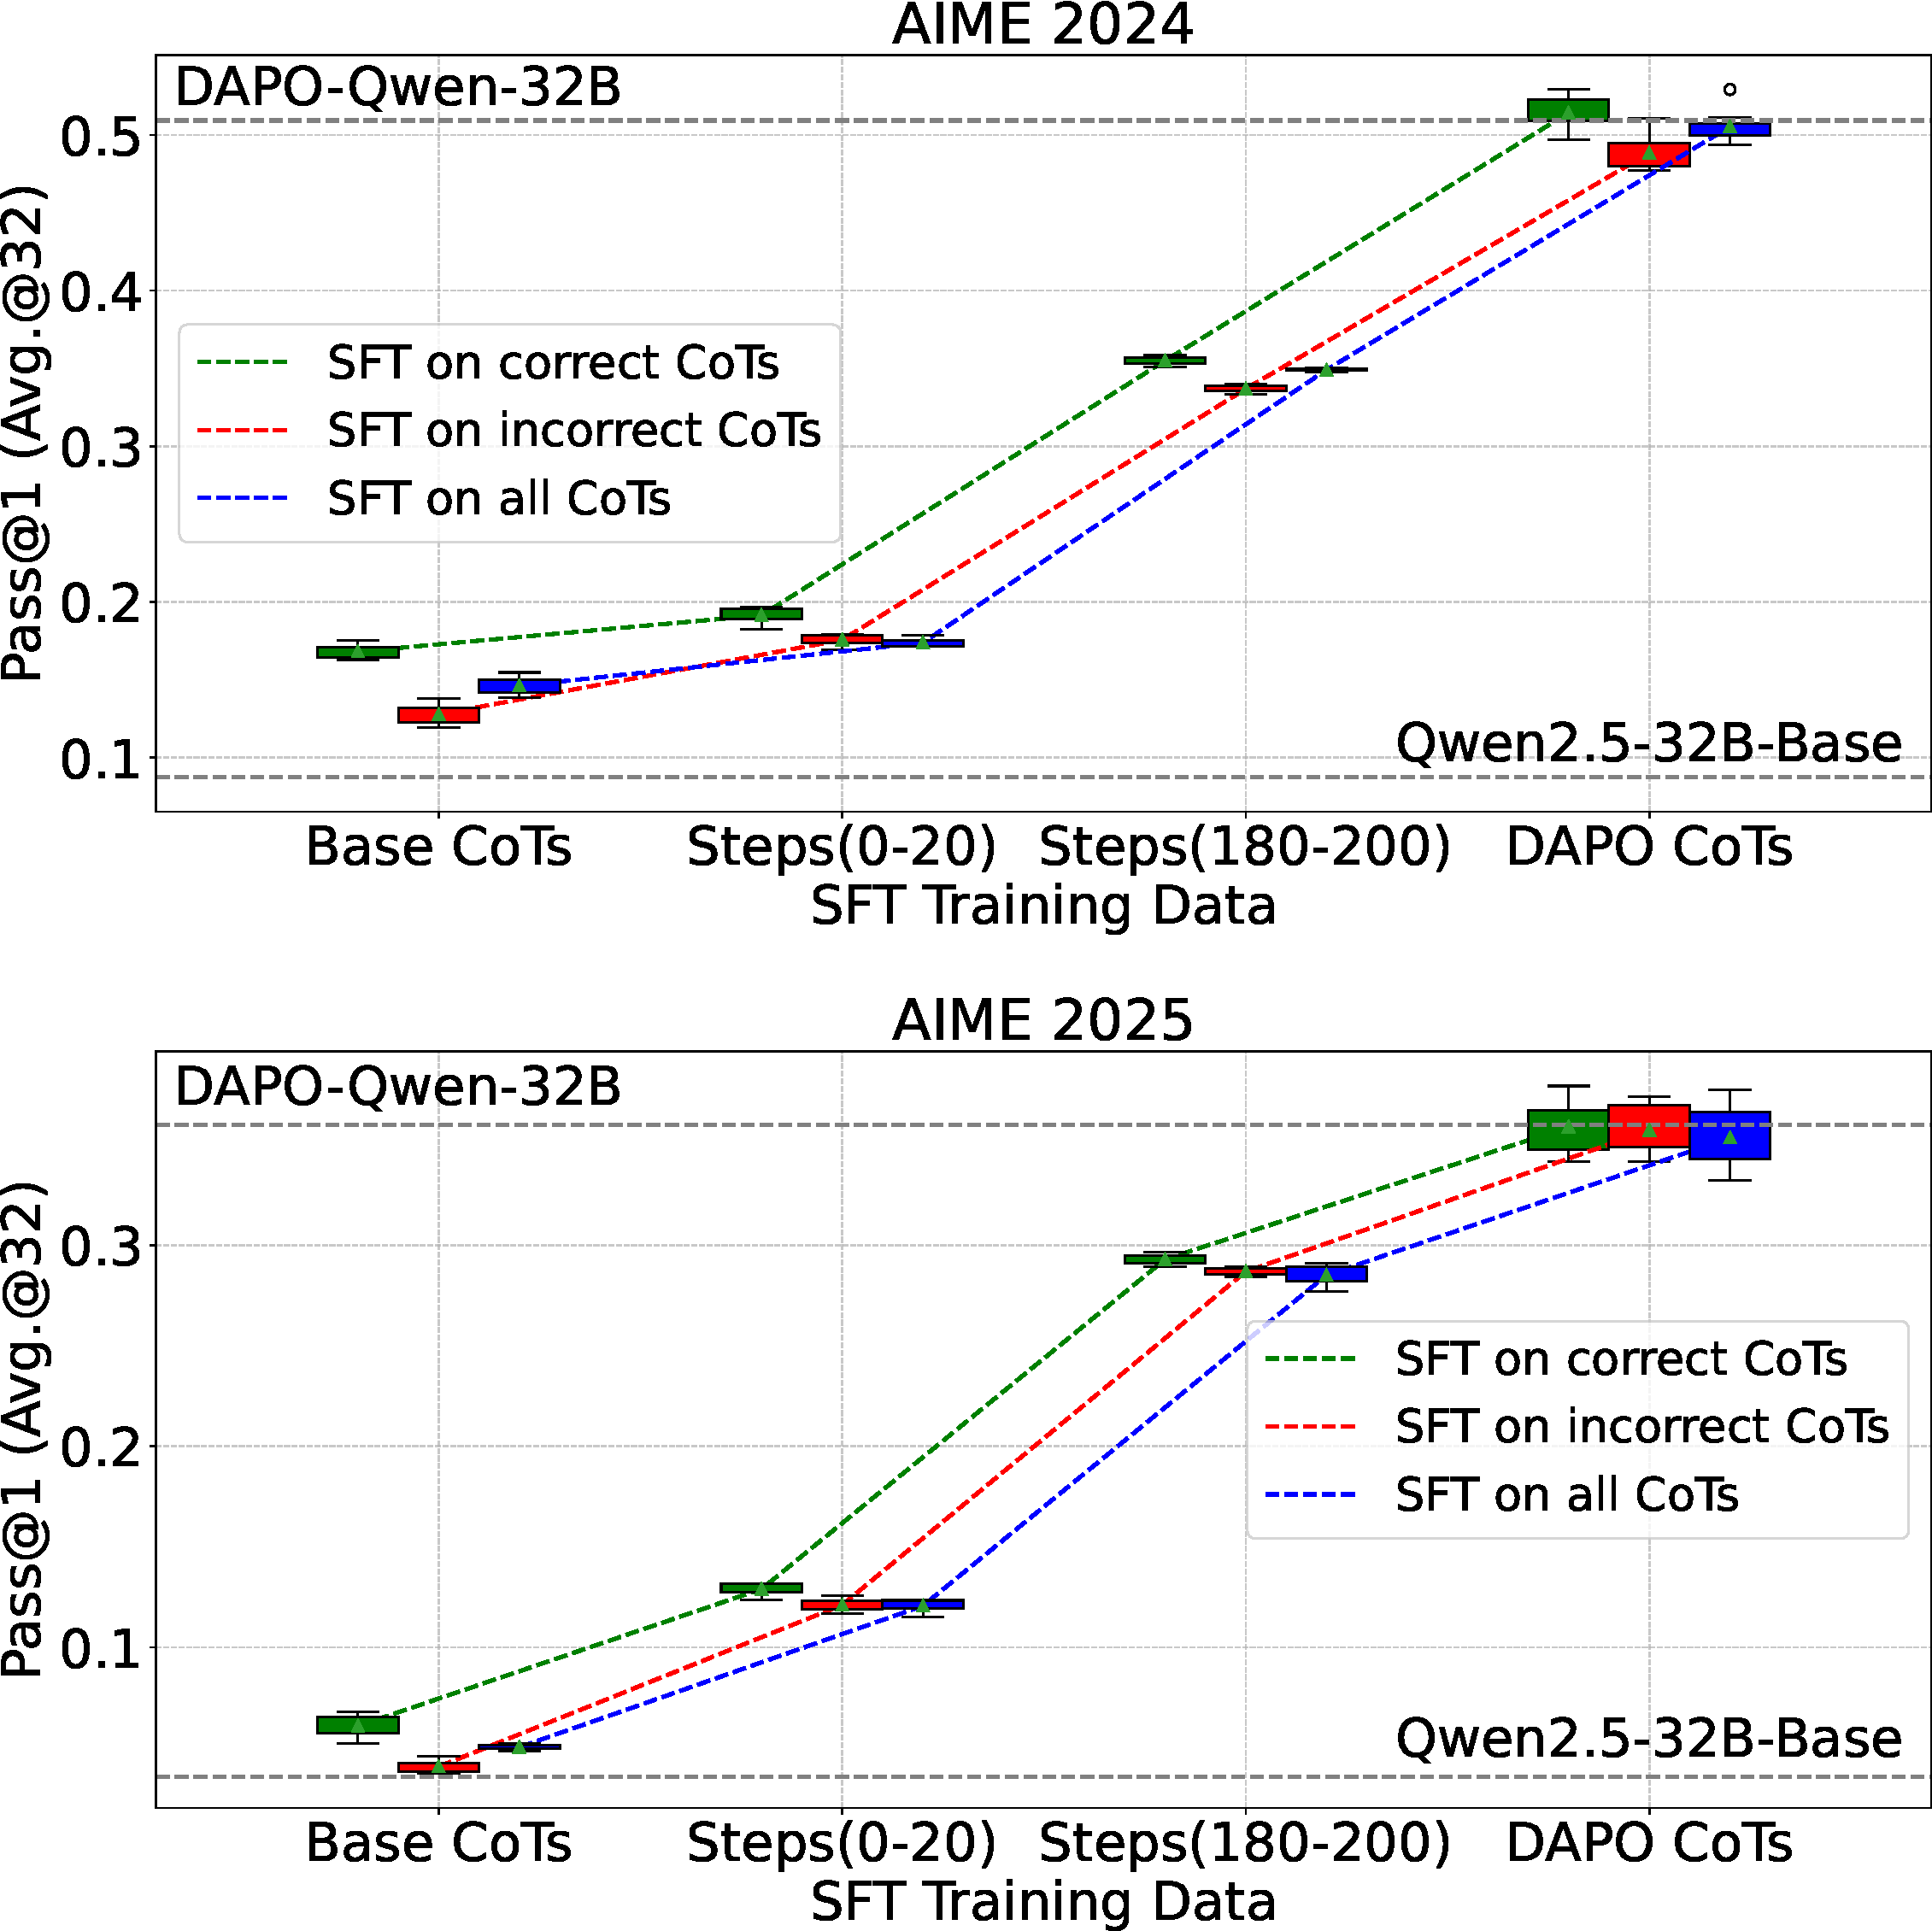
\includegraphics[width=0.48\linewidth]{figures/wxm_comp_sft_data_pass1.pdf}
        \label{fig:comp_sft_data_pass1}
    }
    % \\
    % \vspace{-5pt}
    \hspace{-1pt}
    \subfigure[
        The CoT quality before and after RLVR, using (CoT-)Pass@K on test sets as the proxy metric.
    ]{
        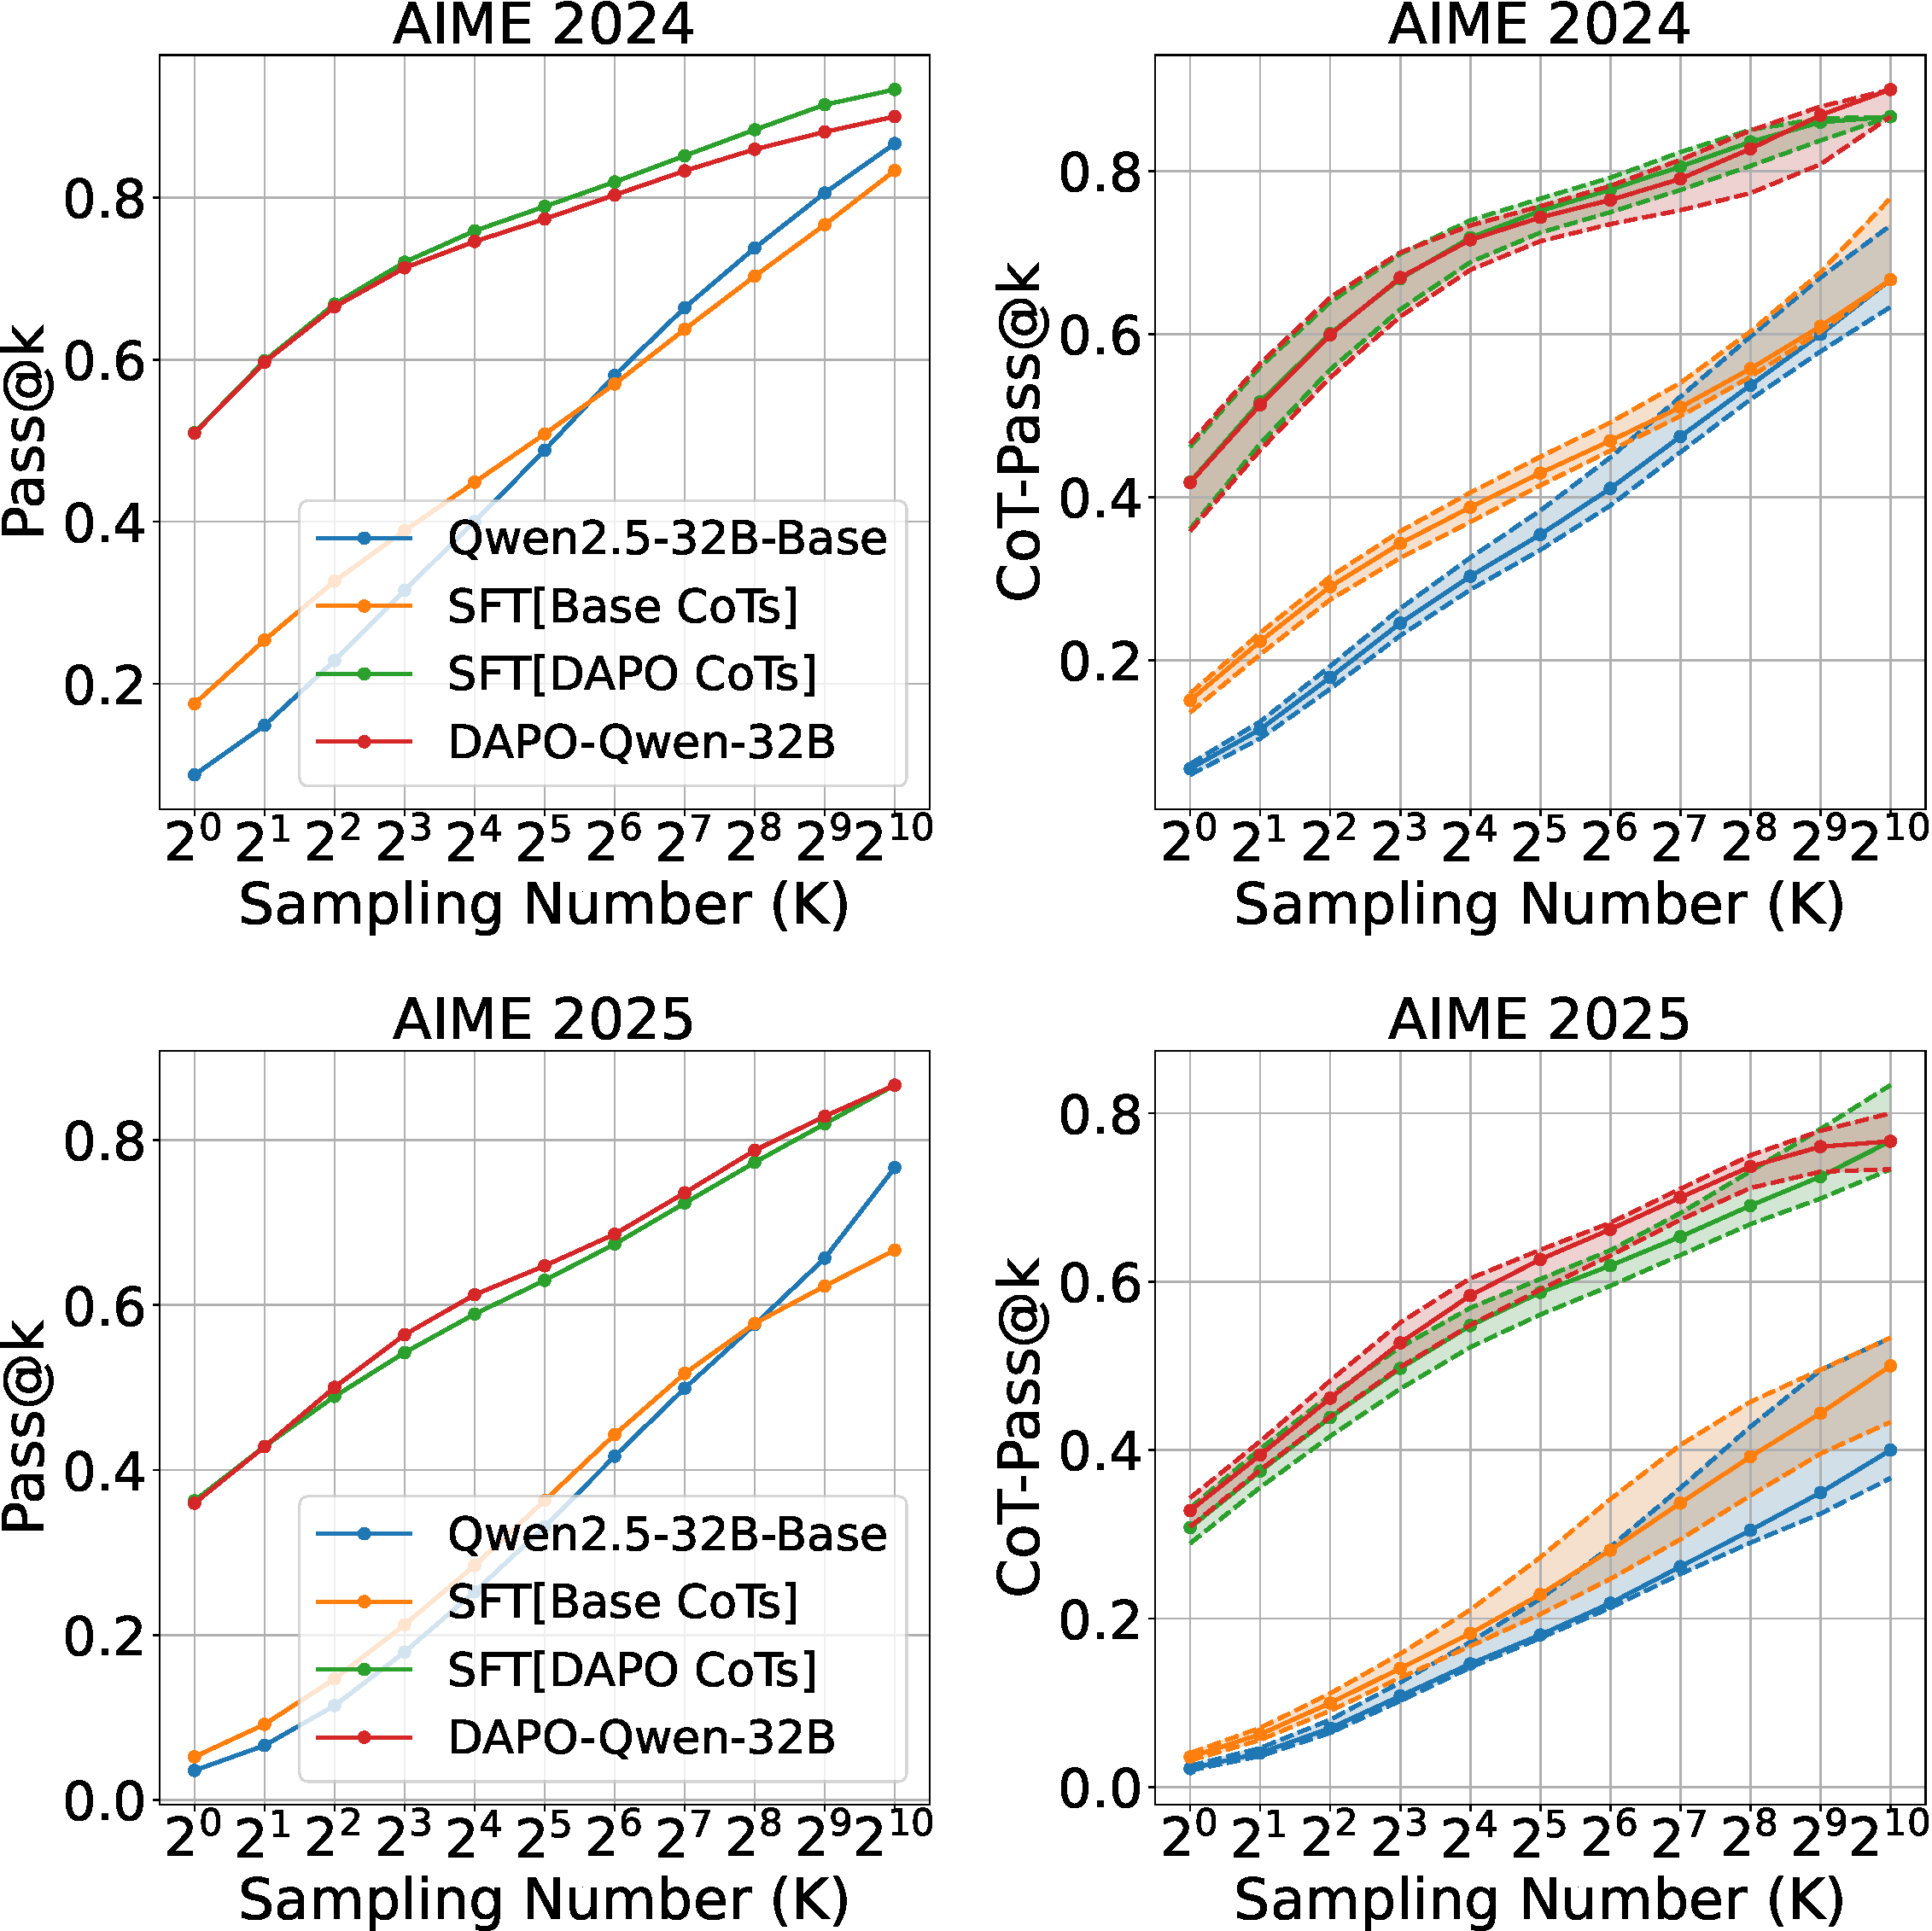
\includegraphics[width=0.48\textwidth]{figures/wxm_comp_sft_rlvr_passk.pdf}
        \label{fig:comp_sft_rlvr_passk}
    }
\caption{
We show the generalization performance of post-SFT LLMs optimized on different CoT data. All these SFT processes start from the same base LLM, Qwen2.5-32B, with the only variable being the different CoT data on DAPO training questions. We use the performance on test sets (AIME 2024, 2025) as a proxy for the quality of the corresponding CoT data.
}
\label{fig:cot_quality_analysis}
\end{figure*}

Specifically, Figure~\ref{fig:comp_sft_data_pass1} illustrates the evolution of CoT quality during RLVR. As training progresses, the generalization performance of post-SFT LLMs, measured in Pass@1, improves steadily. Ultimately, SFT on DAPO CoT data matches the Pass@1 performance of DAPO-Qwen-32B. This result indicates that, given sufficient training questions and CoT data from a post-RLVR model, we can replicate a new model with nearly the same Pass@1 performance simply through SFT.
Moreover, an interesting observation is that, regardless of whether the CoT data contains identifiable errors, as RLVR progresses, the CoT quality, measured in Pass@1, generally improves. This suggests that although some erroneous steps may be present, the overall quality of these "incorrect" CoTs in the later stages of RLVR improves significantly.

Figure~\ref{fig:comp_sft_rlvr_passk} compares the CoT quality before and after RLVR, using both Pass@K and CoT-Pass@K as proxy metrics. Comparing DAPO-Qwen-32B with the post-SFT model trained on its CoT data, we observe that this simple SFT approach nearly replicates the performance of a post-RLVR model, which would otherwise require significant computational cost. When comparing Qwen2.5-32B with the post-SFT model trained on its CoT data, we find that the post-SFT model begins to mitigate guessing. This aligns with our expectations, as we only feed CoT data with correct answers from Qwen2.5-32B into the SFT procedure. We can therefore regard this process as a round of off-policy RLVR optimization.
These observations indicate that the incentivized CoT data through RLVR is crucial, as such CoTs cannot be directly sampled from base LLMs. RLVR optimizes the model's reasoning abilities, ensuring that the generated CoTs are more accurate, coherent, and reliable, which is essential for handling complex tasks.


